% Installing the Mech Sketch beta as an app of its own. Compile with XeLaTeX.
\documentclass[10pt,a4paper]{article}
\usepackage[a4paper, margin=16mm, top=14mm, bottom=14mm]{geometry}
\usepackage{fontspec}
\setmainfont{Inter}[UprightFont = *-Regular, BoldFont = *-SemiBold, ItalicFont = *-Italic, BoldItalicFont = *-SemiBoldItalic]
\usepackage{xcolor}
\usepackage{graphicx}
\usepackage[most]{tcolorbox}
\usepackage{enumitem}
\usepackage{tabularx}
\usepackage[hidelinks]{hyperref}

\definecolor{ink}{HTML}{17201B}
\definecolor{ink2}{HTML}{55615A}
\definecolor{board}{HTML}{E7EBE5}
\definecolor{soft}{HTML}{F3F5F1}
\definecolor{softline}{HTML}{C2CABF}
\definecolor{accent}{HTML}{E2570A}
\color{ink}

\setlength{\parindent}{0pt}
\setlength{\parskip}{0pt}
\pagestyle{empty}
\linespread{1.12}

% A key or a menu item, as it is written on screen.
\newcommand{\key}[1]{\tikz[baseline=(k.base)]\node[k, draw=softline, fill=white, rounded corners=2pt, inner sep=1.6pt, inner xsep=3pt, font=\footnotesize](k){#1};}
\tikzset{k/.style={}}
\newcommand{\menu}[1]{\textbf{#1}}
% The browsers' menu buttons: three dots, upright in Chrome and in a row in Edge.
\newcommand{\vdotsbtn}{\tikz[baseline=-0.65ex]{\foreach \y in {-0.15,0,0.15} \fill (0,\y) circle (0.8pt);}}
\newcommand{\hdotsbtn}{\tikz[baseline=-0.65ex]{\foreach \x in {-0.15,0,0.15} \fill (\x,0) circle (0.8pt);}}
\newcommand{\step}[1]{\tikz[baseline=(s.base)]\node[circle, fill=accent, text=white, inner sep=0pt, minimum size=17pt, font=\bfseries\small](s){#1};}
\newtcolorbox{panel}[1][]{enhanced, colback=soft, colframe=soft, boxrule=0pt, arc=4pt, left=8pt, right=8pt, top=7pt, bottom=7pt, boxsep=0pt, before upper={\raggedright}, #1}
\newcommand{\head}[1]{{\large\bfseries #1}\par\vspace{5pt}}

\begin{document}

% ---------- Title ----------
\begin{minipage}[c]{0.74\linewidth}\raggedright
  {\fontsize{20}{24}\selectfont\bfseries Install the beta as its own app}\par\vspace{5pt}
  {\color{ink2}Mech Sketch beta in a window of its own, with its own desktop icon, beside the released app. It takes about a minute in Chrome or Edge.}
\end{minipage}\hfill
\begin{minipage}[c]{0.22\linewidth}\raggedleft
  
\includegraphics[height=17mm]{icon-512.png}\hspace{3mm}
\includegraphics[height=17mm]{icon-beta-512.png}\par\vspace{2pt}
  {\scriptsize\color{ink2}released app\hspace{6.5mm}beta}
\end{minipage}

\vspace{7pt}
{\color{softline}\rule{\linewidth}{0.6pt}}
\vspace{6pt}

% ---------- What you get ----------
\begin{panel}
  \head{What you get}
  \small
  \begin{itemize}[leftmargin=12pt, itemsep=1pt, topsep=0pt, label={\color{accent}\textbullet}]
    \item An app called \textbf{Mech Sketch beta}, with the orange \textbf{b} on its icon, in its own window, on the desktop and in the Start menu.
    \item It runs beside the released app; installing it changes nothing about the released one.
    \item It keeps its own sketch: work in one never shows up in the other.
  \end{itemize}
\end{panel}

\vspace{5pt}

% ---------- Steps ----------
{\large\bfseries Steps}\par\vspace{6pt}

\begin{tabularx}{\linewidth}{@{}p{7mm}X@{}}
  \step{1} & \textbf{Open the beta in Chrome or Edge:} \href{https://mech-sketch.org/beta/}{\textbf{mech-sketch.org/beta/}}\par
            {\color{ink2}\small The address ends in \texttt{/beta/}. Without it, you get the released app.}\\[5pt]
  \step{2} & \textbf{Load the newest version:} press \key{Ctrl}\,+\,\key{Shift}\,+\,\key{R} \;{\color{ink2}\small(\key{Cmd}\,+\,\key{Shift}\,+\,\key{R} on a Mac).}\\[5pt]
  \step{3} & \textbf{Check that it is the beta:} the orange \textbf{beta} tag is beside the name, top left.\par\vspace{4pt}
            
\includegraphics[height=7.2mm]{header-beta.png}\\[5pt]
  \step{4} & \textbf{Install it.} Click the \textbf{install icon} at the right end of the address bar, then \menu{Install}. Or use the browser's menu:\par\vspace{3pt}
            \begin{tabular}{@{}ll@{}}
              \small Chrome & \small \vdotsbtn\enspace›\, \menu{Cast, save, and share} \,›\, \menu{Install page as app…}\\
              \small Edge & \small \hdotsbtn\enspace›\, \menu{Apps} \,›\, \menu{Install this site as an app}\\
            \end{tabular}\par\vspace{4pt}
            \begin{tcolorbox}[enhanced, colback=white, colframe=accent!55, boxrule=0.6pt, arc=3pt, left=6pt, right=6pt, top=4pt, bottom=4pt, boxsep=0pt, before upper={\raggedright\small}]
              \textbf{Released app already installed?} Then Chrome offers only \emph{Open in Mech Sketch} instead of installing. Use\enspace\vdotsbtn\enspace›\, \menu{Cast, save, and share} \,›\, \menu{Create shortcut…}, name it \textbf{Mech Sketch beta}, tick \menu{Open as window} and choose \menu{Create}.
            \end{tcolorbox}\\[5pt]
  \step{5} & \textbf{Done.} The beta opens in its own window. Next time, start it from its icon on the desktop or in the Start menu.\par
            {\color{ink2}\small No desktop icon? In Chrome, open \texttt{chrome://apps}, right-click \emph{Mech Sketch beta} and choose \menu{Create shortcuts…}}\\
\end{tabularx}

\vspace{5pt}

% ---------- Bottom row ----------
\begin{tcbraster}[raster columns=3, raster equal height=rows, raster column skip=7pt,
  enhanced, colback=soft, colframe=soft, boxrule=0pt, arc=4pt, left=7pt, right=7pt, top=7pt, bottom=7pt, boxsep=0pt, before upper={\raggedright\small}]
  \begin{tcolorbox}
    \head{Keeping it up to date}
    The beta updates itself: each time it starts online, it loads the newest version that has been published. If something looks out of date, press \key{Ctrl}\,+\,\key{Shift}\,+\,\key{R} in its window.\par\vspace{4pt}
    To see which version you have, open \textbf{View settings} (the sliders, top right). The last line says when it was built.\par\vspace{5pt}
    \centering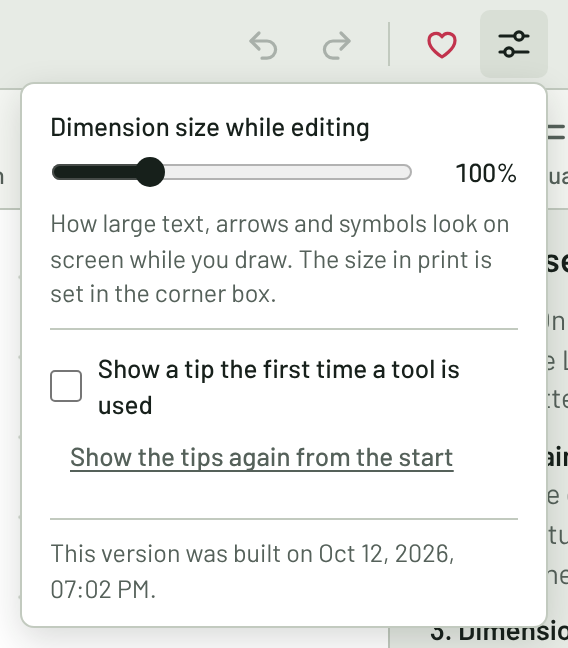
\includegraphics[width=0.5\linewidth]{view-settings.png}
  \end{tcolorbox}
  \begin{tcolorbox}
    \head{Sketches and files}
    Each app keeps its own sketch in the browser, so the two never overwrite each other.\par\vspace{4pt}
    \textbf{Save} and \textbf{Open} work in both. A file saved in the beta with something new in it, such as a plot or a spring, may not show those parts when it is opened in the released app, until they are released.
  \end{tcolorbox}
  \begin{tcolorbox}
    \head{Removing it}
    In the beta's window, open the menu at the top right and choose \menu{Uninstall Mech Sketch beta}. The released app stays.\par\vspace{4pt}
    Or right-click it on \texttt{chrome://apps} (\texttt{edge://apps} in Edge) and remove it there.\par\vspace{6pt}
    \head{On a Mac}
    Chrome and Edge work the same way. Safari can do it too: \menu{File} \,›\, \menu{Add to Dock}.
  \end{tcolorbox}
\end{tcbraster}

\vfill
{\color{softline}\rule{\linewidth}{0.6pt}}\par\vspace{4pt}
{\small\color{ink2}Released app: \href{https://mech-sketch.org}{mech-sketch.org} \hfill Beta: \href{https://mech-sketch.org/beta/}{mech-sketch.org/beta/} \hfill Problems? The report button, top right in the app}

\end{document}
